% FitDash — Training Copilot: architecture graph (standalone, crops to the figure).
% Build:  latexmk -pdf fitdash-architecture-graph.tex
\documentclass[border=12pt]{standalone}
\usepackage[T1]{fontenc}
\usepackage[sfdefault]{FiraSans}   % Inter-like sans, matches the app
\usepackage{xcolor}
\usepackage{tikz}
\usetikzlibrary{positioning,arrows.meta,fit,backgrounds,calc}

% ── FitDash palette ───────────────────────────────────────────────────────────
\definecolor{fdNavy}{HTML}{0B1219}
\definecolor{fdSlate}{HTML}{16212B}
\definecolor{fdBorder}{HTML}{1E293B}
\definecolor{fdTeal}{HTML}{2DD4BF}
\definecolor{fdTealDark}{HTML}{14B8A6}
\definecolor{fdMuted}{HTML}{64748B}

\begin{document}
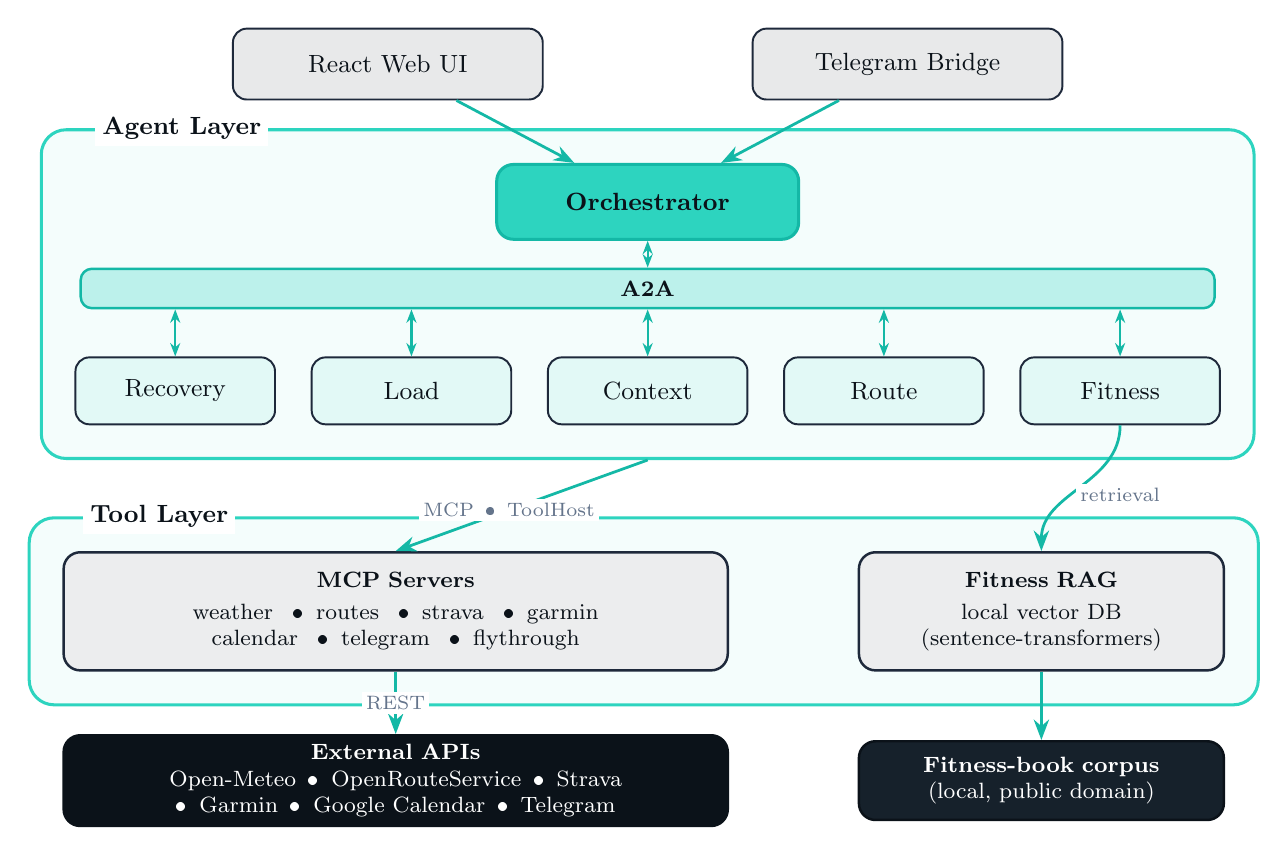
\begin{tikzpicture}[
  font=\sffamily,
  client/.style={rounded corners=5pt, draw=fdBorder, line width=0.7pt, fill=fdSlate!10,
                 text=fdNavy, align=center, font=\small, text width=3.7cm, minimum height=0.9cm},
  orch/.style={rounded corners=6pt, draw=fdTealDark, line width=1.1pt, fill=fdTeal,
               text=fdNavy, align=center, font=\small\bfseries, text width=3.6cm, minimum height=0.95cm},
  agent/.style={rounded corners=5pt, draw=fdBorder, line width=0.7pt, fill=fdTeal!14,
                text=fdNavy, align=center, font=\small, text width=2.3cm, minimum height=0.85cm},
  bus/.style={rounded corners=4pt, draw=fdTealDark, line width=0.9pt, fill=fdTeal!32,
              text=fdNavy, font=\footnotesize\bfseries, minimum width=14.4cm, minimum height=0.5cm},
  comp/.style={rounded corners=6pt, draw=fdBorder, line width=0.9pt, fill=fdSlate!8,
               text=fdNavy, align=center, font=\footnotesize},
  ext/.style={rounded corners=6pt, draw=fdNavy, line width=0.9pt, fill=fdNavy,
              text=white, align=center, font=\footnotesize},
  group/.style={rounded corners=9pt, draw=fdTeal, line width=1.1pt, fill=fdTeal!5, inner sep=12pt},
  ltitle/.style={font=\bfseries\small, text=fdNavy, fill=white, inner sep=2.5pt},
  flow/.style={-{Stealth[length=2.6mm]}, line width=1.0pt, draw=fdTealDark},
  link/.style={{Stealth[length=1.7mm]}-{Stealth[length=1.7mm]}, line width=0.8pt, draw=fdTealDark},
  elabel/.style={font=\scriptsize, text=fdMuted, fill=white, inner sep=1.5pt},
]

% ── Clients ───────────────────────────────────────────────────────────────────
\node[client] (cweb) at (-3.3,0) {React Web UI};
\node[client] (ctg)  at ( 3.3,0) {Telegram Bridge};

% ── Agent layer: orchestrator + specialists on a shared A2A bus ───────────────
\node[orch] (orch) at (0,-1.75) {Orchestrator};
\node[bus]  (bus)  at (0,-2.85) {A2A};
\node[agent] (arec)   at (-6,-4.15) {Recovery};
\node[agent] (aload)  at (-3,-4.15) {Load};
\node[agent] (actx)   at ( 0,-4.15) {Context};
\node[agent] (aroute) at ( 3,-4.15) {Route};
\node[agent] (afit)   at ( 6,-4.15) {Fitness};

% bus connections (double-headed = peer-to-peer A2A)
\draw[link] (orch.south)  -- (orch.south  |- bus.north);
\foreach \a in {arec,aload,actx,aroute,afit}{ \draw[link] (\a.north) -- (\a.north |- bus.south); }

% ── Tool layer: MCP servers component + Fitness RAG component ─────────────────
\node[comp, text width=8.2cm, minimum height=1.5cm] (mcp) at (-3.2,-6.95)
  {\textbf{MCP Servers}\\[2pt]weather \, \textbullet \, routes \, \textbullet \, strava \, \textbullet \, garmin
   \\ calendar \, \textbullet \, telegram \, \textbullet \, flythrough};
\node[comp, text width=4.4cm, minimum height=1.5cm] (rag) at (5.0,-6.95)
  {\textbf{Fitness RAG}\\[2pt]local vector DB\\(sentence-transformers)};

% ── External data ─────────────────────────────────────────────────────────────
\node[ext, text width=8.2cm, minimum height=1.0cm] (extapi) at (-3.2,-9.1)
  {\textbf{External APIs}\\Open-Meteo \,\textbullet\, OpenRouteService \,\textbullet\, Strava \,\textbullet\,
   Garmin \,\textbullet\, Google Calendar \,\textbullet\, Telegram};
\node[ext, text width=4.4cm, minimum height=1.0cm, fill=fdSlate] (corpus) at (5.0,-9.1)
  {\textbf{Fitness-book corpus}\\(local, public domain)};

% ── Layer grouping boxes (drawn behind) ──────────────────────────────────────
\begin{scope}[on background layer]
  \node[group, fit=(orch)(bus)(arec)(afit)] (AL) {};
  \node[group, fit=(mcp)(rag)] (TL) {};
\end{scope}
\node[ltitle, anchor=west] at ($(AL.north west)+(0.7,0)$) {Agent Layer};
\node[ltitle, anchor=west] at ($(TL.north west)+(0.7,0)$) {Tool Layer};

% ── Flows between layers ──────────────────────────────────────────────────────
\draw[flow] (cweb) -- (orch);
\draw[flow] (ctg)  -- (orch);
\draw[flow] (AL.south) -- (mcp.north) node[elabel, pos=0.55]{MCP \,\textbullet\, ToolHost};
\draw[flow] (afit.south) to[out=-90,in=90] (rag.north);
\node[elabel] at ($(afit.south)!0.55!(rag.north)+(0.55,0)$){retrieval};
\draw[flow] (mcp.south) -- (extapi.north) node[elabel, pos=0.5]{REST};
\draw[flow] (rag.south) -- (corpus.north);

\end{tikzpicture}
\end{document}
